 \chapter{Metodologia}
 
Este capítulo apresenta a estrutura geral do sistema, que se divide em duas partes. A primeira parte consiste no \textit{backend} desenvolvido em Python com o objetivo de reconhecer as \textit{tags} utilizando técnicas de \textit{Machine Learning}. A segunda parte consiste na aplicação \textit{web}, desenvolvida em Node.JS, responsável pela visualização e gerenciamento do sistema através de relatórios e telas.

A validação do projeto será feita através de um sistema que seja capaz de identificar números localizados em etiquetas em uma única imagem.

%------------------------------------------------

\section{Visão geral do sistema} \label{sec:funcionamento}

Esta seção descreve as características operacionais do sistema, assim como as respostas esperadas. O fluxo geral do sistema pode ser visualizado na Figura \ref{fig:arqgeral}.

\begin{figure}[htbp]
	\centering
	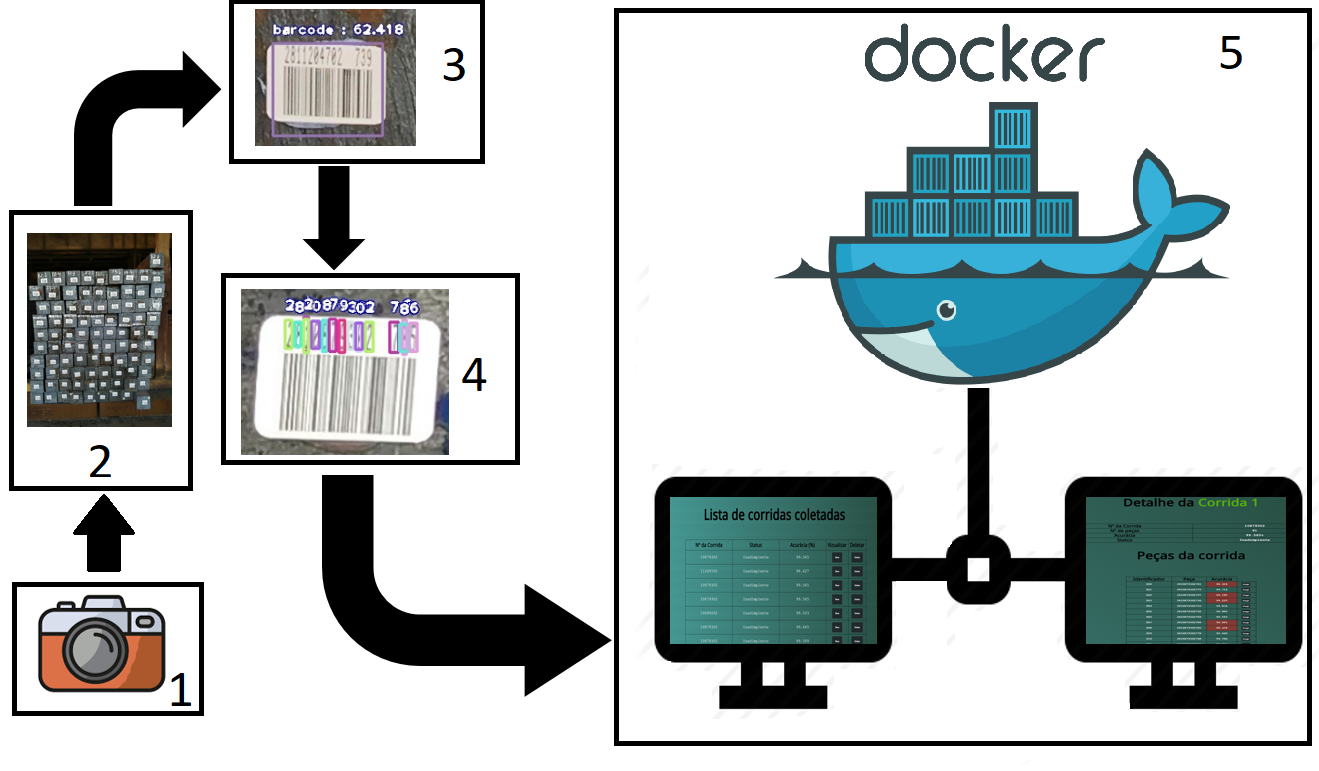
\includegraphics[width=1\linewidth]{capitulos/FluxoDoProjeto.png}
	\caption{Arquitetura geral do projeto.}
	\begin{tabular}{r@{: }l r@{: }l}
    1 & Câmera Fotográfica & 4 & Identificação de números \\
    2& Foto das peças da corrida & 5 & Aplicação WEB \\
    3 & Identificação dos códigos de  barra
    \end{tabular}
	\label{fig:arqgeral}
\end{figure}

Utilizando uma câmera fotográfica, a primeira etapa consiste em fotografar as peças de uma corrida no despacho. A partir dessa fotografia, o código de barras de cada tarugo será reconhecido, e posteriormente, os números que estão acima dele. Essas corridas serão salvas em um banco de dados e mostrados através de telas para que o usuário possa validá-las.

%------------------------------------------------

\section{Backend em Python} \label{sec:backend}

Para realizar o experimento é necessário treinar um modelo de rede neural que seja capaz de reconhecer código de barras e algarismos. Para isso, são efetuadas três etapas. Primeiro será coletado o maior número possível de imagens dos códigos de barras. Em seguida, é gerado um \textit{dataset} com as características dessas imagens junto com a classe em que pertence. Então, é possível realizar a configuração e treinamento da rede neural. E por fim será calculada a acurácia, mediante imagens de teste, do modelo que teve a melhor performance no treinamento.

Escolhemos prioritariamente a linguagem de programação Python para implementação do sistema de Machine Learning devido à grande comunidade existente da linguagem, ao grande número de bibliotecas de análise de dados disponiveis e à ferramenta Google Colab utiliza-ló.

%------------------------------------------------

\subsubsection*{Python}

Python é uma linguagem de programação interpretada\footnote{Linguagem interpretada é uma linguagem de programação em que o código fonte nessa linguagem é executado por um programa de computador chamado interpretador, que em seguida é executado pelo sistema operacional ou processador.}, de alto nível, ou seja,com um nível de abstração relativamente elevado e de uso geral. Sua abordagem orientada a objetos têm como objetivo ajudar os programadores a escrever código para projetos de pequena e grande escala.

O Python suporta vários paradigmas de programação, incluindo programação estruturada (principalmente processual), orientada a objetos e funcional.

Os interpretadores de Python estão disponíveis para muitos sistemas operacionais. Uma organização sem fins lucrativos, a Python Software Foundation, gerencia e direciona recursos para o desenvolvimento do Python. \cite{van2007python}

%------------------------------------------------

\subsection{Preparação do dataset}

Como o escopo do trabalho não contempla a automatizacão da recuperacão de informacões de \textit{websites} públicos, foi disponibilizado um repositório com imagens. Esse
repositório possui 500 imagens e foi disponibilizado pelo laboratório Applied Recognition Technology Laboratory. As imagens se tratam de diferentes tipos de códigos de barras.\cite{Arte-Lab}

\begin{figure}[htbp]
	\centering
	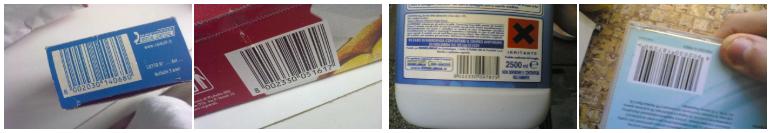
\includegraphics[width=1\linewidth]{figuras/MachineLearning/barcodes.png}
	\caption{Dataset dos código de barras}
	\label{fig:datasetBarcode}
\end{figure}

Para que possamos treinar um modelo de rede neural com alta taxa de acerto, é ideal que tenhamos o maior número possível de imagens no \textit{dataset}. Com isso, foi utilizado o método de \textit{data augmentation} para aumentar a quantidade de imagens que já tínhamos disponíveis. Como iremos utilizar uma rede já pré treinada, utilizaremos em média 1000 imagens em nossa rede.

%------------------------------------------------

\subsubsection*{\textit{Data Augmentation}}\label{sec:dataAugm}

\textit{Data Augmentation} é o processo de aumentar a quantidade e a diversidade de dados de forma sintética. A partir uma imagem, ele pode gerar mais imagens semelhantes através de vários métodos como girar um ângulo qualquer, embaçar a imagem fazendo com que ela perca o brilho ou até mesmo ofuscando-a, entre outros para que possa aumentar o tamanho do \textit{dataset}.

Mesmo quando os dados são de qualidade inferior como, por exemplo, imagens não nítidas, os algoritmos de ML podem ter um desempenho melhor, desde que dados úteis possam ser extraídos pelo modelo do conjunto de dados original. Por exemplo, os modelos de conversão de texto em fala e em texto melhoraram devido ao lançamento de um corpus\footnote{Um corpus pode ser entendido como uma coleção de porções de texto selecionadas de acordo com um conjunto de critérios para representar, tanto quanto possível, uma determinada língua \cite{sinclair2005corpus}} de trilhões de palavras pelo Google \cite{halevy2009unreasonable}. Esse resultado ocorre apesar dos dados serem coletados de páginas da Web não filtradas e conter muitos erros.\cite{dataAug}

O uma parte do código \ref{cod:dataaug} do método mostra o momento em que é definido o tipo de ação que será feita em cada foto, como rotacionar em um ângulo aleatório, inserir ruído na imagem e girar horizontalmente. O método também possibilita escolher a quantidade de imagens que será gerada, neste caso, 1000 imagens.

\begin{lstlisting}[caption=Exemplo de código do método \textit{data augmentation}, label=cod:dataaug][htb!]
 num_files_desired = 1000
 available_transformations = {
                                'rotate': random_rotation,
                                'noise': random_noise,
                                'horizontal_flip': horizontal_flip
                             }
\end{lstlisting}

%------------------------------------------------

\subsection{Anotações das imagens}

Após ter criado o dataset, teremos que fazer as anotações das imagens geradas. Isso quer dizer, criar um arquivo que contenha as posições dos pixels da \textit{Bounding Box} que engloba o objeto na imagem. Um dos formatos mais conhecidos é o Pascal VOC. O formato VOC do Pascal usa arquivos XML para armazenar as informações sobre os objetos anotados nas imagens. Para que possamos gerar esse arquivos mais facilmente, utilizaremos o software LabelImg para realizar essa tarefa.

%------------------------------------------------

\subsubsection*{\textit{Bounding Box}}

A \textit{Bounding Box}(bbox) (Figura \ref{fig:boundingBox}) é um dos métodos de anotação de imagem mais populares usados em \textit{Machine Learning} e em \textit{Deep Learning}.

Elas são caixas retangulares que podem ser determinadas pelo recorte da imagem baseado nas coordenadas das extremidades. Com exemplo, definiremos as \textit{Bounding Boxes} do cachorro e do gato com base nas informações de coordenadas da imagem superior na Figura \ref{fig:boundingBox}. \cite{allDeep}

\begin{figure}[htbp]
		\centering
		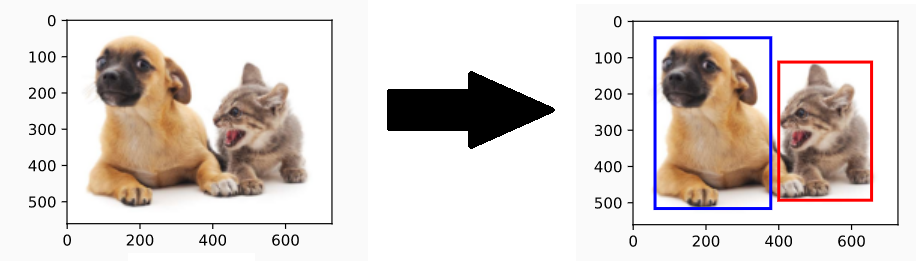
\includegraphics[scale=0.6]{figuras/MachineLearning/catDog.png}
		\caption{Execução de \textit{Bounding Boxes}.}
		\legend{Fonte: \cite{133Ob9905723:online})}
		\label{fig:boundingBox}
\end{figure}

O código \ref{cod:bbox} refere-se à posição das \textit{Bounding Boxes} do cachorro e do gato na imagem, respectivamente.

\begin{lstlisting}[caption=Posições de X e Y nas \textit{Bounding Boxes}, label=cod:bbox]
         dog_bbox, cat_bbox = [60, 45, 378, 516], [400, 112, 655, 493]
\end{lstlisting}

%------------------------------------------------

\subsubsection*{LabelImg}\label{sub:LabelImg}

O LabelImg (Figura \ref{fig:labelimg}) é uma ferramenta \textit{open source} de anotação de imagem gráfica escrita em Python. As anotações são salvas em arquivos XML no formato PASCAL VOC (Código \ref{cod:XML}), o formato usado pelo ImageNet. Além disso, também suporta o formato YOLO no qual utilizaremos em nosso projeto. \cite{labelimg}

O software em questão permite que você circule as \textit{bounding boxes} englobando o objeto de interesse nas imagens e criando automaticamente um arquivo XML com todas as especificações necessárias.

Utiliza-se a ferramenta para formar o \textit{dataset}, que é um dos fundamentos da \textit{Deep Learning}. Para muitos pesquisadores, obter dados suficientes para realizar o experimento por si só é um grande problema, por isso precisamos de muitos \textit{datasets open source} para que todo mundo possa usar. Alguns \textit{datasets} comumente usados na visão computacional são os seguintes.

\begin{figure}[htbp]
	\centering
	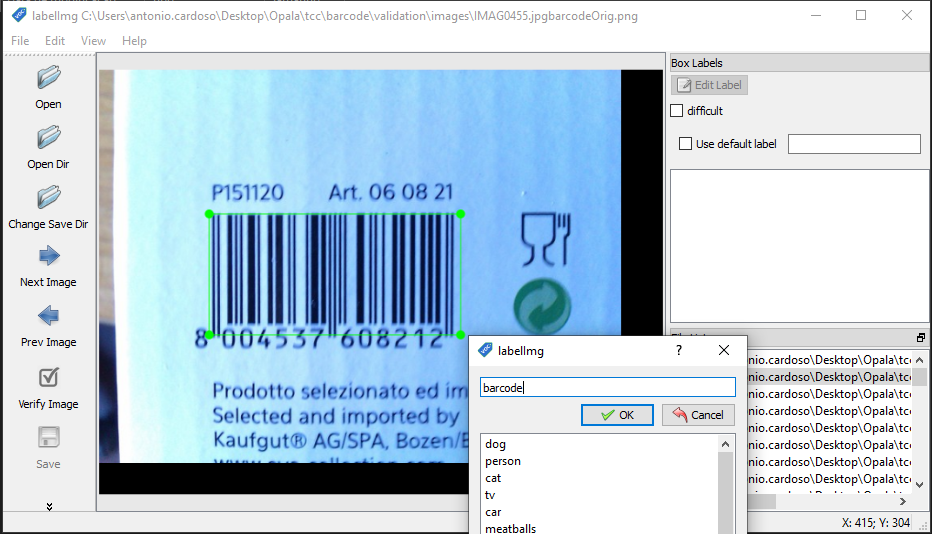
\includegraphics[width=0.9\linewidth]{figuras/MachineLearning/labelimg.png}
	\caption{Procedimento de anotações das \textit{bounding boxes}}
	\label{fig:labelimg}
\end{figure}

\begin{lstlisting}[caption=Arquivo XML gerado pelo LabelImg, label=cod:XML]
<annotation>
	<folder>images</folder>
	<filename>05102009081.jpgbarcodeOrig.png</filename>
	<path>C:\Users\antonio.cardoso\Desktop\tcc\barcode\train\images\05102009081.jpgbarcodeOrig.png</path>
	<source>
		<database>Unknown</database>
	</source>
	<size>
		<width>640</width>
		<height>480</height>
		<depth>3</depth>
	</size>
	<segmented>0</segmented>
	<object>
		<name>barcode</name>
		<pose>Unspecified</pose>
		<truncated>0</truncated>
		<difficult>0</difficult>
		<bndbox>
			<xmin>105</xmin>
			<ymin>63</ymin>
			<xmax>536</xmax>
			<ymax>454</ymax>
		</bndbox>
	</object>
</annotation>
\end{lstlisting}

O ImageNet dataset \cite{deng2009imagenet} possui mais de 14 milhões de imagens, cobrindo mais de 20.000 categorias. Existem mais de um milhão de imagens com anotações explícitas de classe e anotações de locais de objetos na imagem. O conjunto de dados Imagenet é um dos conjuntos de dados mais usados no campo da \textit{Deep Learning}. A maior parte do trabalho de pesquisa, como classificação, localização e detecção de imagens, é baseada nesse conjunto de dados. O conjunto de dados Imagenet é detalhado e é muito fácil de usar. É amplamente utilizado no campo da pesquisa em visão computacional e se tornou o conjunto de dados 'padrão' do aprendizado profundo atual do domínio da imagem para testar o desempenho do algoritmo. \cite{zhou2017application}

\subsubsection*{PASCAL VOC}
O PASCAL VOC (análise de padrões, modelagem estatística e classes de objetos visuais de aprendizado computacional) \cite{everingham2010pascal} fornece conjuntos de dados de imagem padronizados para reconhecimento de classe de objetos e fornece um conjunto comum de ferramentas para acessar os conjuntos de dados e anotações. O conjunto de dados PASCAL VOC inclui 20 classes e tem um desafio baseado nesse conjunto de dados. O PASCAL VOC Challenge \cite{everingham2010pascal} não está mais disponível após 2012, mas seu conjunto de dados é de boa qualidade e bem marcado e permite a avaliação e comparação de diferentes métodos. E como a quantidade de dados do conjunto de dados PASCAL VOC é pequena, comparada ao conjunto de dados imagenet, muito adequada para os pesquisadores testarem programas de rede. Nosso conjunto de dados também é criado com base no padrão de conjunto de dados PASCAL VOC.\cite{zhou2017application}

Depois de ter feito as anotações para todas as imagens, será necessário separar o conjunto de teste e treinamento. Criaremos uma pasta o dataset chamada barcodes e dentro dela, será criada também uma pasta de nome \textbf{train} e \textbf{validation}.

Para o treinamento, separamos o conjunto de teste para que não possua nenhuma imagem presente no conjunto de treinamento. O \textit{dataset} de testes terá uma amostra bem menor que o conjunto de treinamento, portanto terá mais ou menos 25\% do total das imagens.

Depois de fazer isso, a estrutura da pasta do  \textit{dataset} de  \textit{barcodes} será a seguinte:

\begin{figure}[htbp]
	\centering
	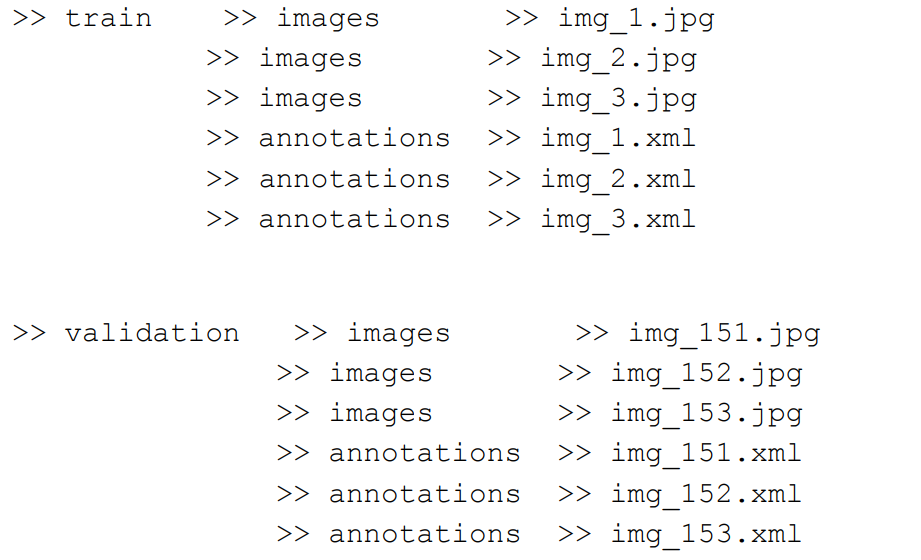
\includegraphics[width=0.5\linewidth]{figuras/MachineLearning/foldersDataset.png}
	\caption{Estrutura de pastas do \textit{dataset} de barcodes}
	\label{fig:labelimg}
\end{figure}

Ou seja, para cada imagem, teremos um arquivo XML com as anotações registradas pelo Labelimg. Agora poderemos treinar nossos modelos.

%------------------------------------------------

\subsection{Infraestrutura}

Com o intuito de acelerar o processo, foi utilizado um software online chamado Google Colaboratory que tem disponibilidade de configuração com GPU para o treinamento. 

%------------------------------------------------

\subsubsection{Google Colaboratory}
O Google Colaboratory, mais conhecido como "Google Colab" ou simplesmente "Colab", é um projeto de pesquisa para criar protótipos de modelos de \textit{Machine Learning} em poderosas opções de \textit{hardware}, como GPUs e TPUs. Ele fornece um ambiente de notebook Jupyter sem servidor para desenvolvimento interativo. O Google Colab é gratuito para usar como outros produtos do G Suite — que anteriormente era conhecido como Google Apps — no qual é um serviço oferecido pelo Google que fornece diversas ferramentas da própria empresa. Elas podem ser totalmente personalizadas com as informações do negócio, incluindo um domínio próprio.

Além de ser fácil de usar, o Colab é muito flexível em sua configuração e faz muito do trabalho pesado para você. \cite{colabdetail}

\begin{itemize}
    \item Suporte para Python 2.7 e Python 3.6;
    \item Aceleração de GPU;
    \item Bibliotecas pré-instaladas: Todas as principais bibliotecas Python, como o TensorFlow, o Scikit-learn, o Matplotlib, entre muitas outras, estão pré-instaladas e prontas para serem importadas;
    \item Construído com base no Jupyter Notebook;
    \item Recurso de colaboração (funciona com uma equipe igual ao Google Docs): o Google Colab permite que os desenvolvedores usem e compartilhem o Jupyter notebook entre si sem precisar baixar, instalar ou executar qualquer coisa que não seja um navegador;
    \item Suporta comandos \textit{bash};
    \item Os notebooks do Google Colab são armazenados no drive.
\end{itemize}

\begin{figure}[htbp]
		\centering
		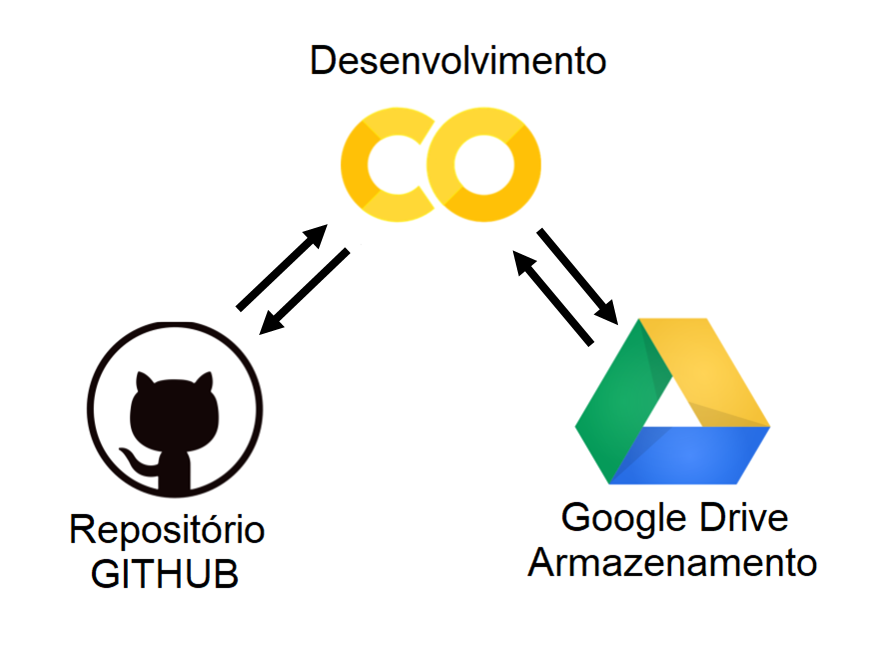
\includegraphics[scale=0.4]{figuras/MachineLearning/colabGithub.png}
		\caption{Utilização do Colab, Drive e Github}
		\label{fig:colabGithub}
\end{figure}

O Colab se integra facilmente ao Google Drive, o que o torna uma opção natural para espaço de armazenamento, em que se armazena os dados e os modelos. Ao mesmo tempo, o Github é mais adequado para hospedagem de código e uso de diversas  bibliotecas gratuitas disponíveis pela comunidade. 

\subsection{Blibliotecas utilizadas}

Todo o código foi implementado utilizando a linguagem de programacão Python, e as seguintes bibliotecas foram utilizadas:

%------------------------------------------------

\subsubsection{TensorFlow}

O TensorFlow é uma biblioteca Python de código aberto para implementar algoritmos de \textit{Machine Learning}. Um código utilizando o TensorFlow pode ser executado com pouca ou nenhuma alteração em uma ampla variedade de sistemas heterogêneos, desde dispositivos móveis como telefones e tablets até sistemas distribuídos em larga escala de centenas de máquinas e milhares de dispositivos computacionais, como placas de GPU.

O sistema é flexível e tem sido usado para conduzir pesquisas e implantar sistemas de aprendizado de máquina na produção em mais de uma dúzia de áreas da ciência da computação e outros campos, incluindo reconhecimento de fala, visão computacional, robótica, recuperação de informações, processamento de idiomas, extração de informações geográficas e descoberta computacional de drogas. \cite{abadi2016tensorflow}

Vários serviços do Google uilizam o TensorFlow em sua produção, foi lançado como um projeto de código aberto e tornou-se amplamente utilizado para pesquisa de ML.\cite{199317}

%------------------------------------------------

\subsubsection{Scikit-Image}

O Scikit-image, também conhecido como Skimage, é uma biblioteca de processamento de imagens que implementa algoritmos e utilitários para uso em aplicações de pesquisa, educação e indústria. É lançado sob a licença liberal de código aberto Modified BSD, fornece uma API bem documentada na linguagem de programação Python e é desenvolvido por uma equipe internacional ativa de colaboradores.

O objetivo do scikit-image é fornecer uma biblioteca de alta qualidade de ferramentas poderosas e diversas de processamento de imagens, gratuitas e sem restrições. Esses princípios são a base para as práticas de desenvolvimento na comunidade de imagens scikit.\cite{skimage}

%------------------------------------------------

\subsubsection{ImageAI}

ImageAI é uma biblioteca python de código aberto criada para capacitar os desenvolvedores a criar aplicativos e sistemas com recursos independentes de \textit{Deep Learning} e \textit{Computer Vision} usando poucas linhas de código.

A biblioteca ImageAI suporta previsão e treinamento de imagens usando 4 algoritmos diferentes de \textit{Machine Learning} treinados no conjunto de dados ImageNet-1000. O ImageAI também suporta detecção de objetos, detecção de vídeo e rastreamento de objetos usando RetinaNet, YOLOv3 e TinyYOLOv3 treinados no conjunto de dados COCO e PASCAL VOC.\cite{ImageAI}

Neste trabalho será utilizada uma classe da biblioteca ImageAI chamada \textit{Custom Detection Model Training}, possibilitando o treinamento do meu próprio modelo de detecção de objetos utilizando a arquitetura da YOLOv3.

%------------------------------------------------

\subsubsection{OpenCV}

O OpenCV (Open Source Computer Vision) é uma biblioteca de \textit{open source} e \textit{cross-plataform} (Multiplataforma) que contém mais de 500 algoritmos otimizados para análise de imagem e vídeo. Desde sua introdução em 1999, ele foi amplamente adotado como a principal ferramenta de desenvolvimento pela comunidade de pesquisadores e desenvolvedores em visão computacional.\cite{opencv}

%------------------------------------------------

\subsection{Treinamento dos modelos}

Após gerado o conjunto de dados, é possível trabalhar no treinamento do modelo da rede neural. Para isso será utilizado o \textit{framework} TensorFlow destinado à \textit{Deep Learning}. Também será utilizado uma rede neural pré-treinada chamada YoloV3, escrita em Python que fará uso das funções disponibilizadas pela biblioteca ImageAI . Assim realizando o treinamento até atingir um valor aceitável de acerto no conjunto de teste. 

Através do modelo da rede Yolov3, treinaremos mais dois novos modelos de redes neurais:
\begin{itemize}
    \item Modelo de rede neural para reconhecimento de \textit{barcodes};
    \item Modelo de rede neural para reconhecimento de algarismos numéricos;
\end{itemize}

O resultado do treinamento serão arquivos no formato .h5\footnote{Um arquivo H5 é um arquivo de dados salvo no formato \textit{Hierarchical Data Format}(HDF). Contém conjuntos multidimensionais de dados científicos.} representando o modelo que serão avaliados através da melhor acurácia\footnote{Indica uma performance geral do modelo. Dentre todas as classificações, quantas o modelo classificou corretamente;} e utilizados posteriormente.

%------------------------------------------------

\subsubsection*{YOLOv3}\label{sub:Yolov3}

A rede neural YOLOv3 evoluiu de YOLO e YOLO-V2 \cite{redmon2018yolov3}. Quando comparado com a rede Faster R-CNN, a mais eficiente das CNNs quando, a YOLO transforma o problema de detecção em um problema de regressão, em que a informação tem um significado numérico resultante de alguma previsão na imagem. Isto não requer uma região da proposta e gera coordenadas e probabilidades de \textit{bounding boxes} (\textit{bbox}) de cada classe diretamente por meio de regressão. Isso aumenta consideravelmente a velocidade de detecção em comparação com o Faster R-CNN.\cite{yolov3_apple}

O YOLO é a frequência mais rápida (45 FPS) do que outros algoritmos de detecção de objetos \cite{yolov3RealTime}. Comparando a rede Faster R-CNN com a  R-CNN, a velocidade do treinamento  é 9 vezes mais rápida e a velocidade do teste é 213 vezes mais rápida. \cite{7960069}

O YOLO impõe fortes restrições espaciais nas previsões de \textit{bbox}, pois cada célula da \textit{grid} prevê apenas duas \textit{box} e pode ter apenas uma classe. Essa restrição espacial limita o número de objetos próximos que o modelo pode prever. O modelo luta com pequenos objetos que aparecem em grupos, como por exemplo, bandos de pássaros. \cite{yolov3RealTime}

\begin{figure}[htbp]
		\centering
		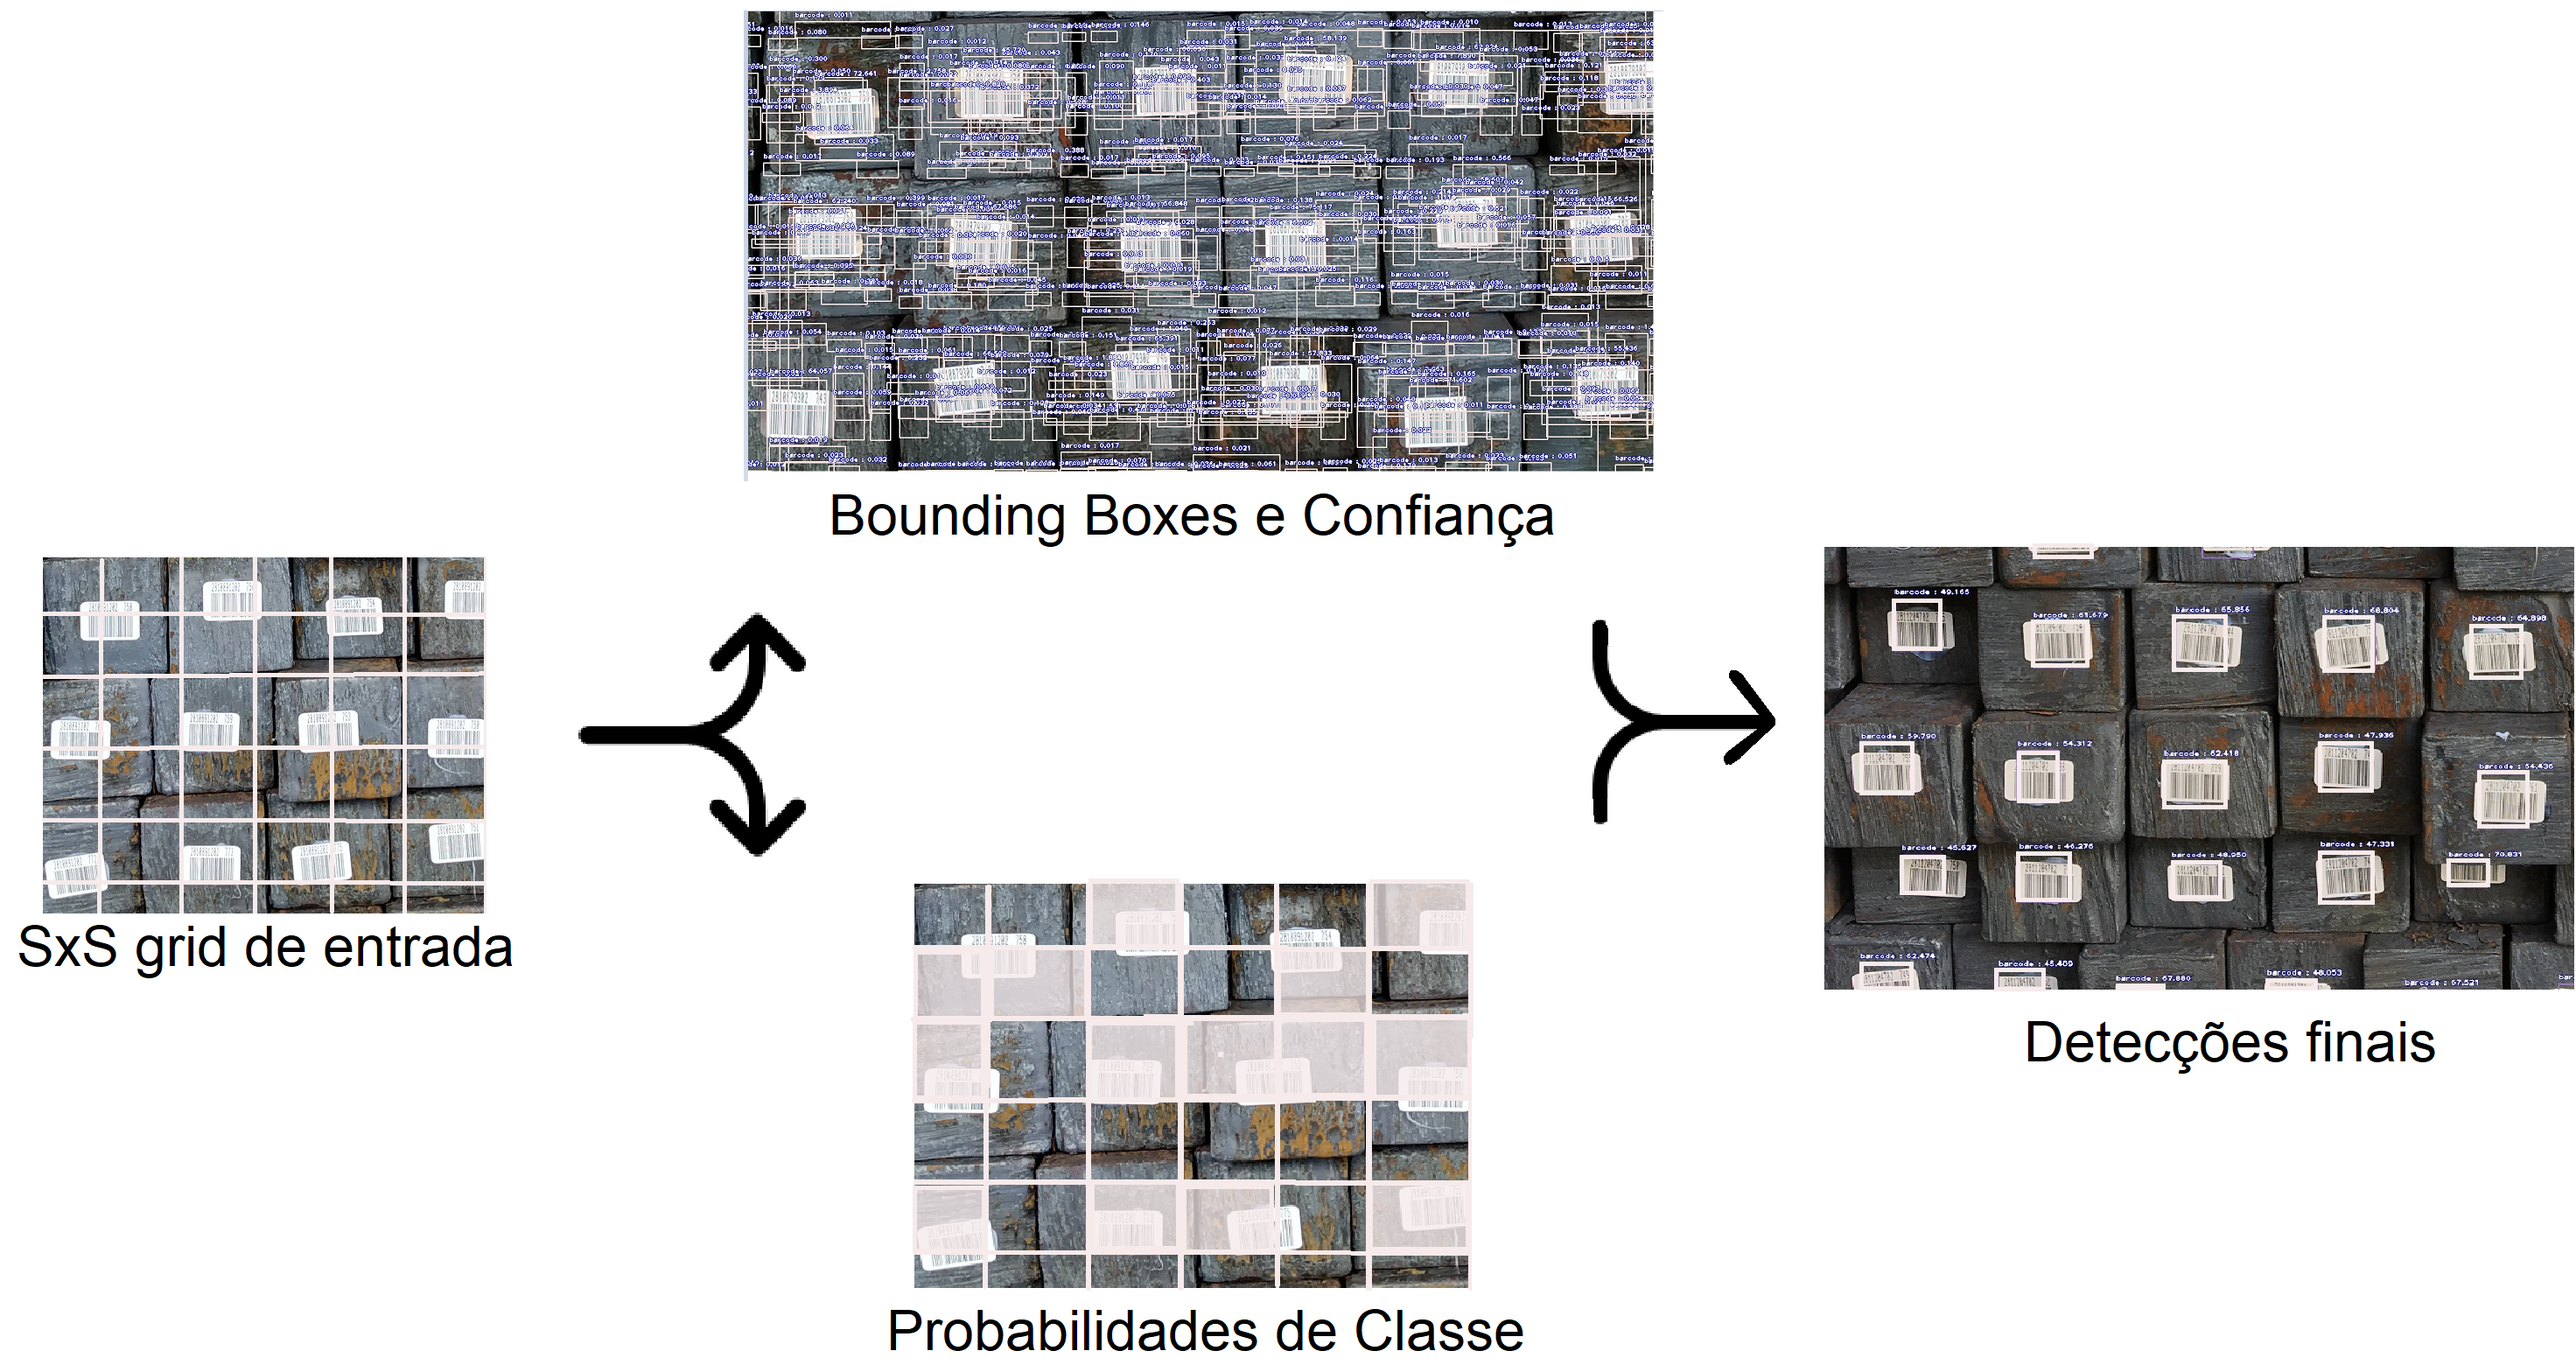
\includegraphics[scale=0.2]{figuras/MachineLearning/yolo.png}
		\caption{YOLO}
		\label{fig:yolo}
\end{figure}

No modelo de detecção YOLO (Figura \ref{fig:yolo}) uma única rede convolucional prediz tanto os \textit{bounding boxes} quanto as probabilidades de pertinencia a classe de cada objeto detectado. Para isso, YOLO funciona da seguinte forma:

\begin{itemize}
    \item Toma-se uma imagem e divide-se-a em um grid SxS de células (S = 6);
    \item Usando o \textit{grid} como referência, gera-se N \textit{bounding boxes};
    \item \textit{Bounding boxes} com probabilidade acima de um limiar são selecionados e usados para localizar o objeto dentro da imagem.
\end{itemize}

Cada célula do  \textit{grid} é usada para predizer B  \textit{bbox} e C probabilidades de classe. O conceito de interseção sobre união (IoU) tem um papel importante e a confiança de uma predição em YOLO é dada por:

\begin{equation}
    Confianca = p_r(Object) X IoU_{pred}^{truth} , p_r(Object) \in \left \{ 1\right.,\left.0\right \}
\end{equation}

Em que, quando o \textit{target} estiver na \textit{grid}, \(p_r(Object)\) = 1 e 0 caso contrário. \(IoU_{pred}^{truth}\) é usado para denotar a interseção sobre união e a previsão da \textit{bbox}. A confiança reflete se a \textit{grid} contém objetos e a precisão da \textit{bbox} prevista. Quando várias \textit{bbox} detectam o mesmo \textit{target}, o YOLO usa o método de não supressão máxima (NMS) para selecionar a melhor \textit{bbox}.

%------------------------------------------------

\section{Aplicação Web} \label{sec:web}

Neste seção mostraremos as etapas necessárias de criação da aplicação web desenvolvida para consumir os resultados do sistema de \textit{Deep Learning} mostrado anteriormente. 

O sistema web foi criado para facilitar o gerenciamento, visualização e rastreabilidade das corridas para o operador através de um \textit{layout} amigável.

Para essa etapa, utilizaremos a linguagem Node.JS para implementar o \textit{back-end} e as linguagens HTML, CSS, EJS\footnote{O EJS é uma engine de visualização, com ele conseguimos de uma maneira fácil e simples transportar dados do back-end para o front-end, basicamente conseguimos utilizar códigos em javascript no html de nossas páginas.} e JavaScript para implementar o \textit{front-end}. A escolha do Node.JS foi devido aos seguintes fatores:

\begin{itemize}
    \item Instalação ser simples pois não necessita de dependência para configuração
    \item Você consegue executar aplicações Node em qualquer plataforma.
    \item I/O não bloqueante. Isso significa que quando você precisa acessar um arquivo no disco, se comunicar com um \textit{Web Service} ou acessar um banco de dados esse acesso é feito de forma assíncrona por padrão.
    \item Por ser escrito em JavaScript, pouparia grande parte dos esforço caso opte por utilizar tecnologias \textit{front-end}, que na maioria, também são escritas em JavaScript.
\end{itemize}
 
%------------------------------------------------

\subsection{Node.JS}

O Node.JS, também conhecido como Node, é uma estrutura EDA\footnote{Maneira de realizarmos a comunicação entre sistemas que consiste, principalmente em operações assíncronas além de permitir aplicativos escalonáveis e gerar menos acoplamento entre os serviços, permitindo uma arquitetura fortemente flexível.} de código aberto para o desenvolvimento de aplicativos JavaScript em servidores. É baseado no \textit{runtime} do Google, chamado de motor V8. O V8 e o Node são implementados em C e C++, focados no desempenho e baixo consumo de memória. Embora o V8 suporte principalmente o uso de JavaScript no navegador, o Node foca no suporte de processos de servidores \cite{Tilkov2010}.

O Node é um dos \textit{frameworks} mais famosos que suportam o desenvolvimento de servidores utilizando o JavaScript \cite{Tilkov2010}.

%------------------------------------------------

\subsection{HTML}

Para publicar informações para distribuição global, é preciso uma linguagem universalmente compreendida. A linguagem de publicação usada pela WWW\footnote{WWW é um sistema de documentos dispostos na Internet que permitem o acesso às informações apresentadas no formato de hipertexto.} é HTML (da HyperText Markup Language).\citeauthor{html}

O HTML fornece aos autores os meios para: 
\begin{itemize}
    \item Publicar documentos on-line com títulos, texto, tabelas, listas, fotos, etc. 
    \item Recuperar informações on-line por meio de links de hipertexto, com o clique de um botão. 
    \item Criar formulários para realizar transações com serviços remotos, para uso em busca de informações, reservas, pedidos de produtos, etc. 
    \item Incluir planilhas, videoclipes, clipes de som e outros aplicativos diretamente em seus documentos.
\end{itemize}

%------------------------------------------------

\subsection{CSS}
De acordo com \citeauthor{css}, um dos padrões fundamentais do W3C \footnote{Trata-se de uma organização internacional responsável pelos protocolos e padronização da WWW, a rede mundial de computadores.} para o desenvolvimento de aplicativos da web é o \textit{Cascading Style Sheets}(CSS) \cite{Casca8378199:online}. CSS é uma linguagem para definir a semântica de apresentação dos elementos HTML, incluindo seu posicionamento, layout, cor e fontes. A principal mecanismo por trás da adoção do CSS tem sido a separação da estrutura da apresentação. Embora essa separação de preocupações ajude a evolução de um aplicativo da Web no que diz respeito à estrutura e ao conteúdo, o código CSS em si não é fácil de manter.\cite{badros1999constraint}

Escrever código CSS não é trivial \cite{quint2007editing}. Requer interação humano-computador, design gráfico, além de habilidades de programação na web \cite{keller2010css}. Além disso, a linguagem possui várias características, como especificidade de herança, cascata e seletor, o que torna o entendimento de como as propriedades CSS são aplicadas aos elementos DOM em tempo de execução, uma tarefa assustadora para desenvolvedores da web.

%------------------------------------------------

% \subsection{Docker}

% Docker é um projeto \textit{open source} que foi inicialmente lançado em 2013, atraiu grande atenção na industria de TI. É uma plataforma de conteinerização que possibilita usuários a construir sua aplicação dentro de um conteiner e transferir conteiners através de máquinas com diferentes sistemas operacionais de um jeito simples. \cite{chang2017kubernetes}

% Existem três componentes principais do Docker:

% \begin{itemize}
% 	\item \textit{Docker images}: são \textit{templates} de leitura que servem como base para a criação de conteiners.;
% 	\item \textit{Docker registries}: é o local onde estão uma grande coleção de \textit{Docker images}.;
% 	\item \textit{Docker containers}: são as instâncias virtuais em que as aplicações estão rodando. Cada conteiner contem uma aplicação rodando e todas os seus arquivos de dependências, como o código, bibliotecas e utilitários do sistema.
% \end{itemize}

% A construção de imagens pode ser feita de duas maneiras. É possível criar um conteiner através de uma imagem já existente (\textit{docker run}), realizar modificações e instalações dentro do conteiner, parar o container e depois salvar o estado atual do conteiner como uma nova imagem (\textit{docker commit}). Este processo é parecido com uma instalação clássica de uma máquina virtual, mas deve ser feito para cada imagem caso haja alguma atualização, já que as imagens são padronizadas. Para automatizar o processo, \textit{Dockerfiles} nos permite especificar uma imagem de base e uma sequência de comandos que serão executados quando a imagem é construída, juntamente com outras opções de especificações, como portas a serem expostas. A imagem é depois construída com o comando \textit{docker build}.\cite{DiPietro}


%------------------------------------------------
\section{Arquitetura do projeto}

Ao fazer a escolha da arquitetura do projeto, optamos utilizar a arquitetura de \textit{microservices} pois como teremos mais de um módulo de software com linguagens e características diferentes, ficaria mais fácil escalar e fazer manutenções de maneiras independentes.

\subsection{Microsserviços}
Seguindo a definição de \citeauthor{ms1} (\citeyear{ms1}), a arquitetura de microsserviços trata do desenvolvimento de uma aplicação que baseia na existência de diversos pequenos serviços independentes. Cada um dos serviços deve rodar em seu próprio processo independente. Estes serviços podem comunicar entre si utilizando mecanismos leves de comunicação (geralmente em torno no HTTP). Os serviços devem ser absolutamente independentes.

Um exemplo da arquitetura de microsserviços está na Figura \ref{fig:arquitetura-microsservicos}.

\begin{figure}[htbp]
	\centering
	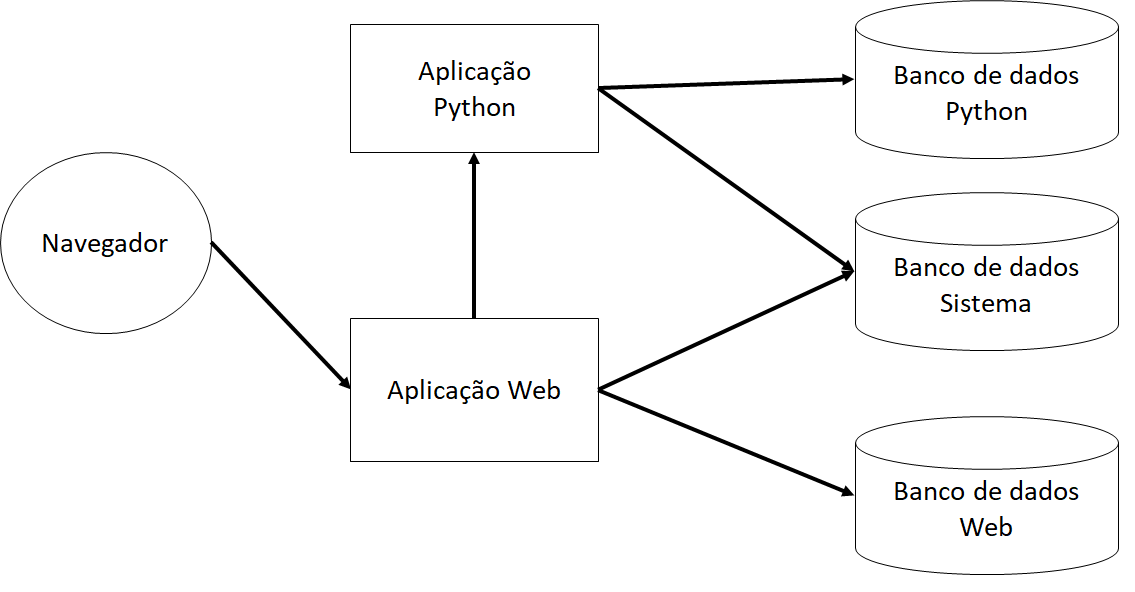
\includegraphics[width=1\linewidth]{figuras/WebService/microservices.png}
	\caption{Exemplo arquitetura de microsserviços.}
	\label{fig:arquitetura-microsservicos}
\end{figure}

Microsserviços são os resultados da decomposição funcional de uma aplicação. São caracterizados pela definição de sua interface e função no sistema. Como cada serviço deve ser independente, uma alteração na sua implementação não deve afetar o funcionamento dos demais. \cite{Pahl}

%------------------------------------------------





